\chapter[Our Framework at Work on the iTrust SWaT System]{Our Framework at Work: Reverse Engineering of the iTrust SWaT System}
\label{application}
\linenumbers

\lettrine{I}{n this} chapter, our main objective is to apply the framework and methodology introduced in Chapter \ref{chap:proposal} to the case study of the iTrust SWaT system, as illustrated in Chapter \ref{casestudy}. The purpose of this analysis is to assess the effectiveness and potential of the proposed framework within the context of a system that closely replicates a real-world water treatment plant, albeit on a smaller scale.

\bigskip
Due to the complexity of the system and the limited space available in this thesis, we will not conduct a comprehensive analysis and reverse engineering of the entire system. Instead, we will focus on specific parts for analysis. We leave it to the reader or those interested in utilizing the proposed methodology and framework to complete the analysis, should they choose to do so.\newline
By focusing on selective components and leaving room for further exploration, we strike a balance between providing valuable insights and acknowledging the potential for additional research. This approach empowers the reader and interested individuals to explore the iTrust SWaT system further and leverage the proposed methodology and framework for a more comprehensive analysis.

\section{Preliminary Operations}
\label{sec:6_preliminar_operations}
Prior to beginning the actual analysis, several preliminary manual operations need to be conducted on the physical process dataset utilized as a case study, specifically the SWaT system dataset for the year 2015 as outlined in Section \ref{subsec:5_2015_datasets}. To simulate the data-capture process performed by Ceccato et al. using their scanning tool, the original dataset in XLSX format (proprietary to Microsoft Excel) was divided into multiple datasets in CSV format. Each of these datasets corresponds to the individual stages of the SWaT system and contains the respective registers. These resulting files were then saved in the directory specified by the \texttt{raw\_dataset\_directory} directive in the framework configuration file, \textit{config.ini}, ready to be used in the pre-processing phase.\newline
Furthermore, the headers were manually renamed by adding a prefix from \texttt{P1\_} to \texttt{P6\_} to each register's name. This prefix indicates the stages, ensuring that each register is easily identifiable and linked to its corresponding stage.

\section{Planning the Analysis Strategy}
\label{sec:6_analysis_strategy}
The complexity of the system being analyzed necessitates the adoption of a deliberate strategy for the analysis. It is not feasible to rely on trial and error or attempt every possible combination between stages. The former approach may overlook crucial relationships between PLCs or between registers, while the latter may result in excessive and unproductive efforts if the specific portion of the system being analyzed lacks significant information or relationships. \newline
A sound analysis strategy helps us focus on the important parts of the system, improving the quality of the analysis and leading to better process comprehension. By prioritizing our attention, we can gain a deeper understanding of the crucial components, resulting in more informed decision-making and a comprehensive understanding of the overall processes.

\bigskip
To define this strategy, a potential starting point could involve analyzing network traffic to determine the communication patterns and participants within the system. This can be accomplished by utilizing the techniques discussed in Section \ref{subsec:4_network_analysis} on Network Analysis. By applying the Python script described in that section to the data extracted from the network traffic dataset debated in Section \ref{par:5_2015_net_dataset}, we can generate a (simplified) network graph, as illustrated in Figure \ref{fig:6_network_SWaT}.

\begin{figure}[ht]
	\centering
	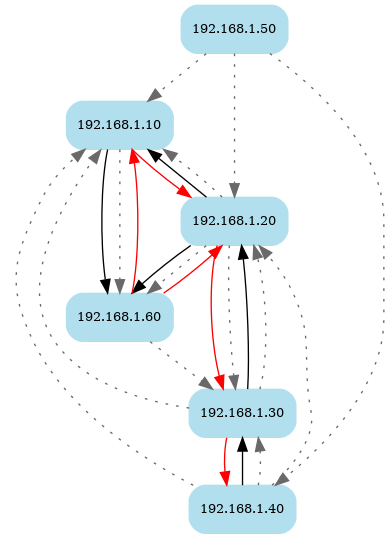
\includegraphics[scale=0.65]{chap6/network2.png}
	\caption{Simplified graph of the iTrust SWaT system network}
	\label{fig:6_network_SWaT}
\end{figure}

The graph clearly illustrates the structure of communications between the PLCs. Referring back to Table \ref{table:5_swat_ip_addresses}, which displays the IP address - PLC associations, we can observe that PLCs 1 through 4 communicate directly and sequentially with each other in a Request/Response communication pattern (represented by red and black arrows, respectively). Additionally, PLC6 communicates with both PLC1 and PLC2. On the other hand, the gray dotted arrows indicate communications for which we have knowledge of a response, but the corresponding request is unknown. For the purposes of our analysis strategy, we will not consider these communications within this context.

\bigskip
Based on our observations, the analysis strategy we will adopt involves considering sequential pairs of PLCs to effectively capture the relationships and implications between registers. Therefore, the PLC pairs we will focus on are PLC1-2, PLC2-3, and PLC3-4. 

\section{Reverse Engineering of the iTrust SWaT System}
\label{sec:6_reverse_SWaT}
Before starting the analysis, it is important to establish a premise regarding how the subsystems under investigation will be defined during the pre-processing phase. Apart from the projection determined by the considered PLCs, a time-based selection of the analysis period has also been performed (see Section \ref{subsubsec:4_select_subsystem}). This selection spans a duration of 20,000 seconds, which is equivalent to approximately five and a half hours or roughly five system cycles. The analysis begins at 100,000 seconds, which corresponds to approximately 27 hours from the start of the available data. This deliberate selection aims to exclude the initial transient period during which the SWaT system is initialized. We believe that this time range is more than sufficient for accurately defining the characteristics of the SWaT system components.

\subsection{Reverse Engineering of PLC1 and PLC2}
\label{subsec:6_P1P2_analysis}
The initial focus of analysis will be on the pair comprising PLC1 and PLC2. In Chapter \ref{chap:proposal}, we have previously discussed certain conjectures and properties concerning PLC1. In this section, we will provide a brief summary of those points before proceeding with the rest of the analysis.

\subsubsection{Pre-processing}
\label{subsubsec:6_P1P2_preprocessing}
After merging the datasets for the two PLCs under investigation, the preliminary analysis performed gives us the outcomes displayed in Listing \ref{lst:6_preproc_P1P2}:

\begin{lstlisting}[language=bash, numbers=left, caption=Preliminary analysis outcomes for sensors and actuators of \texttt{PLC1-2}, label=lst:6_preproc_P1P2]
	Actuators: 
	P1_MV101 [0.0, 1.0, 2.0]
	P1_P101 [1.0, 2.0]
	P2_MV201 [0.0, 1.0, 2.0]
	P2_P203 [1.0, 2.0]
	P2_P205 [1.0, 2.0]
	
	Sensors: 
	P1_FIT101 {'max_lvl': 2.7, 'min_lvl': 0.0}
	P1_LIT101 {'max_lvl': 815.1, 'min_lvl': 489.6}
	P2_AIT201 {'max_lvl': 256.5, 'min_lvl': 252.9}
	P2_AIT202 {'max_lvl': 8.4, 'min_lvl': 8.3}
	P2_AIT203 {'max_lvl': 342.8, 'min_lvl': 320.0}
	P2_FIT201 {'max_lvl': 2.5, 'min_lvl': 0.0}
	
	Hardcoded setpoints or spare actuators: 
	P1_P102 [1.0]
	P2_P201 [1.0]
	P2_P202 [1.0]
	P2_P204 [1.0]
	P2_P206 [1.0]
\end{lstlisting}

Based on the assumptions made in Chapter \ref{chap:proposal}, \texttt{P1\_LIT101} is a \textbf{measurement}. We speculated that \texttt{P1\_LIT101} is likely a \textbf{level sensor for a tank}. This assumption is supported by the wide range of values observed for this sensor, with a minimum value of 489 and a maximum value of 815.
Further \textbf{likely measurements} are available, namely \texttt{P1\_FIT101}, \texttt{P2\_FIT201}, \texttt{P2\_AIT201}, \texttt{P2\_AIT201} and \texttt{P2\_AIT201}. Upon analyzing the range of values for these measurements, it is evident that they do not align with typical characteristics of sensors associated with tanks. At this point, it is challenging to determine the specific association or purpose of these measurements. Further investigation is required to gain clarity on their intended function.

\bigskip
Regarding the actuators, the analysis reveals the following \textbf{likely actuators}: \texttt{P1\_MV101}, \texttt{P1\_P101}, \texttt{P2\_MV201}, \texttt{P2\_P203}, and \texttt{P2\_P205}.\newline
\texttt{P1\_MV101} and \texttt{P2\_MV201} exhibit three states (0, 1, and 2), while \texttt{P1\_P101}, \texttt{P2\_P203}, and \texttt{P2\_P205} operate with two states (1 and 2).\newline
The analysis also indicates the presence of probable \textbf{spare actuators}, which can be identified by their consistent value of 1. This distinguishes them from \textit{relative setpoints}.\newline 
The following spare actuators have been identified: \texttt{P1\_P102}, \texttt{P2\_P201}, \texttt{P2\_P202}, \texttt{P2\_P204}, and \texttt{P2\_P206}.

\noindent Next, we proceed to formalize our observations:

\begin{description}
	\item[\colorbox{backcolourtext}{\normalfont\textit{Conjecture 1:}}] \texttt{P1\_LIT101}, \texttt{P1\_FIT101}, \texttt{P2\_FIT201}, \texttt{P2\_AIT201}, \texttt{P2\_AIT202} and \texttt{P2\_AIT203} are \textbf{measurements}.
	
	\item[\colorbox{backcolourtext}{\normalfont\textit{Conjecture 2:}}] \texttt{P1\_LIT101} is identified as the \textbf{level sensor} specifically associated with a \textbf{tank}.
	
	\item[\colorbox{backcolourtext}{\normalfont\textit{Conjecture 3:}}] \texttt{P1\_MV101}, \texttt{P1\_P101}, \texttt{P2\_MV201}, \texttt{P2\_P203} and \texttt{P2\_MV205} are \textbf{actuators}.
	
	\item[\colorbox{backcolourtext}{\normalfont\textit{Property 1:}}] \texttt{P1\_MV101} and \texttt{P2\_MV201} assume three distinct states, represented by the values 0, 1, and 2.
	
	\item[\colorbox{backcolourtext}{\normalfont\textit{Property 2:}}] \texttt{P1\_P101}, \texttt{P2\_P203} and \texttt{P2\_P205} assume two distinct states, represented by the values 1, and 2.
	
	\item[\colorbox{backcolourtext}{\normalfont\textit{Conjecture 4:}}] \texttt{P1\_102}, \texttt{P2\_P201}, \texttt{P2\_P202}, \texttt{P2\_P204} and \texttt{P2\_P206} are \textbf{spare actuators}.
	
	\item[\colorbox{backcolourtext}{\normalfont\textit{Conjecture 5:}}] a spare actuator in state 1 is considered to be \textbf{OFF}.
	
\end{description}

Continuing with the examination of the outcomes from the preliminary analysis, it is evident that the duration of \texttt{P1\_MV101} and \texttt{P2\_MV201} in state 0 is only a few seconds. However, in the subsequent states, the duration is significantly longer, as demonstrated in Listing \ref{lst:6_preproc_P1P2_time}. 

\begin{lstlisting}[language=bash, numbers=left, caption=Time duration of the states of actuators MV101 and MV201 of PLC1-2, label=lst:6_preproc_P1P2_time]
	Actuator state durations:
	P1_MV101 == 0.0
	9  9  10  9  9  10  9  9  10  9
	
	P1_MV101 == 1.0
	1174  1168  1182  1160  1172
	
	P1_MV101 == 2.0
	669  3019  3012  3000  2981
	
	P2_MV201 == 0.0
	8  8  8  9  9  8  9  9  9  9
	
	P2_MV201 == 1.0
	1057  1057  1045  1038  1039
	
	P2_MV201 == 2.0
	120  3135  3144  3127  3109
\end{lstlisting}

Based on this observation, we can conjecture that state 0 serves as a transient state between the two actual states of the actuator, namely 1 and 2. From this deduction, we formalize the following conjecture:

\begin{description}
	\item[\colorbox{backcolourtext}{\normalfont\textit{Conjecture 6:}}] the state 0 of an actuator is a \textbf{transient state}.
\end{description}

In the analysis of actuator state changes relative to measurements, we referred to examples from Section \ref{subsubsec:4_brief_analysis} that demonstrated the behavior of \texttt{P1\_P101}. We observed that when the actuator state of \texttt{P1\_P101} transitions from 2 to 1, its relative setpoint in relation to \texttt{P1\_LIT101} is approximately 535. Similarly, when the state transitions from 1 to 2, the relative setpoint is approximately 813. Based on these findings, we deduced that \texttt{P1\_P101} is responsible for \textbf{emptying the tank} represented by \texttt{P1\_LIT101}. Moreover, we confirmed our previous assumption that actuator states 1 and 2 correspond to the states of \textbf{OFF and ON, respectively}. Let us now formalize these inferences:

\begin{description}
	\item[\colorbox{backcolourtext}{\normalfont\textit{Conjecture 7:}}] \texttt{P1\_P101} is responsible for \textbf{emptying the tank} represented by \texttt{P1\_LIT101}.
	
	\item[\colorbox{backcolourtext}{\normalfont\textit{Conjecture 8:}}] state 1 of \texttt{P1\_P101} corresponds to the \textbf{OFF state} of the actuator, while state 2 of \texttt{P1\_P101} corresponds to the \textbf{ON state} of the actuator.
	
	\item[\colorbox{backcolourtext}{\normalfont\textit{Property 3:}}] The \textit{relative setpoints} of \texttt{P1\_P101} are approximately 535 (minimum) and approximately 813 (maximum).
\end{description}

The same reasoning applied to \texttt{P1\_P101} can also be applied to \texttt{P1\_MV101}. Listing \ref{lst:6_preproc_P1P2_mv101state} provides a clear representation of the state changes and corresponding relative setpoints for this actuator. 

\begin{lstlisting}[language=bash, numbers=left, caption=\texttt{P1\_MV101} state changes and relative setpoints, label=lst:6_preproc_P1P2_mv101state]
	       P1_LIT101  P1_MV101  prev_P1_MV101
	669     800.7170         0              2
	1850    499.0203         0              1
	4876    800.5992         0              2
	6052    498.9026         0              1
	9071    800.7170         0              2
	10260   499.1381         0              1
\end{lstlisting}

\noindent Once again, let us formalize the observations:
\begin{description}
	\item[\colorbox{backcolourtext}{\normalfont\textit{Conjecture 9:}}] \texttt{P1\_MV101} is responsible for \textbf{filling the tank} represented by \texttt{P1\_LIT101}.
	
	\item[\colorbox{backcolourtext}{\normalfont\textit{Conjecture 10:}}] state 1 of \texttt{P1\_MV101} corresponds to the \textbf{OFF state} of the actuator, while state 2 of \texttt{P1\_MV101} corresponds to the \textbf{ON state} of the actuator.
	
	\item[\colorbox{backcolourtext}{\normalfont\textit{Property 4:}}] The \textit{relative setpoints} of \texttt{P1\_MV101} are approximately 500 (minimum) and approximately 800 (maximum).
\end{description}

To conclude the analysis of PLC1, it is worth examining the behavior of \texttt{P1\_FIT101}, which we previously identified as a flow or pressure sensor. In particular, it is insightful to observe its performance in relation to \texttt{P1\_MV101}, as shown in Listing \ref{lst:6_preproc_P1P2_fit101}.

\begin{lstlisting}[language=bash, numbers=left, caption=\texttt{P1\_FIT101} behavior, label=lst:6_preproc_P1P2_fit101]
	       P1_FIT101  P1_MV101  prev_P1_MV101
	669     2.614419         0              2
	1850    0.000000         0              1
	4876    2.496877         0              2
	6052    0.000000         0              1
	...
		
	       P1_FIT101  P1_MV101  prev_P1_MV101
	677     2.466451         1              0
	4885    2.334497         1              0
	9079    2.396951         1              0
	13276   2.453960         1              0
	17432   2.539154         1              0
	
	       P1_FIT101  P1_MV101  prev_P1_MV101
	1858    1.126413         2              0
	6060    1.112641         2              0
	10269   1.327547         2              0
	14443   0.999263         2              0
	18611   1.140185         2              0
\end{lstlisting}

As observed, \texttt{P1\_FIT101} exhibits values close to 2.5 when the step is made by \texttt{P1\_MV101} from the ON state to the transient state, and values close to 0 when the step is made from the OFF state to the transient state. Notably, when examining the step from the transient state to the OFF and ON states of \texttt{P1\_MV101}, interesting findings emerge. In the former case, a slight decrease in the value of \texttt{P1\_FIT101} can be observed, while in the latter case, the value is just under half.\newline 
Considering these observations collectively, it can be deduced that \texttt{P1\_FIT101} is measuring a flow. Specifically, the flow decreases when the actuator receives a command to close (transition from transient to OFF state), and it increases when the actuator receives a command to open (transition from transient to ON state). \newline 
Based on these deductions, we can speculate that \texttt{P1\_FIT101} is indeed a \textbf{flow sensor}.

\begin{description}
	\item[\colorbox{backcolourtext}{\normalfont\textit{Conjecture 11:}}] \texttt{P1\_FIT101} represents a \textbf{flow sensor}.
\end{description}

\subsubsection{Graphs and Statistical Analysis}
\label{subsubsec:6_P1P2_graphs}

\subsubsection{Invariant Inference and Analysis}
\label{subsubsec:6_P1P2_invariants}

\subsubsection{Business Process Analysis}
\label{subsubsec:6_P1P2_bpa}

\subsection{Reverse Engineering of PLC2 and PLC3}
\label{subsec:6_P2P3_analysis}

\subsubsection{Pre-processing}
\label{subsubsec:6_P2P3_preprocessing}

\subsubsection{Graphs and Statistical Analysis}
\label{subsubsec:6_P2P3_graphs}

\subsubsection{Invariant Inference and Analysis}
\label{subsubsec:6_P2P3_invariants}

\subsubsection{Business Process Analysis}
\label{subsubsec:6_P2P3_bpa}

\subsection{Reverse Engineering of PLC3 and PLC4}
\label{subsec:6_P3P4_analysis}

\subsubsection{Pre-processing}
\label{subsubsec:6_P3P4_preprocessing}

\subsubsection{Graphs and Statistical Analysis}
\label{subsubsec:6_P3P4_graphs}

\subsubsection{Invariant Inference and Analysis}
\label{subsubsec:6_P3P4_invariants}

\subsubsection{Business Process Analysis}
\label{subsubsec:6_P3P4_bpa}

\vfill
\nolinenumbers